\documentclass[11pt,a4paper]{article}
\usepackage[utf8]{inputenc}
\usepackage{amsmath, amssymb}
\usepackage{graphicx}
\usepackage{geometry}
\usepackage{booktabs}
\usepackage{adjustbox}
\usepackage{algorithm}
\usepackage{algorithmic}
\usepackage{hyperref}
\usepackage{caption}
\usepackage{subcaption}
\usepackage{xcolor}
\usepackage{float}

\geometry{margin=1in}

\title{\textbf{Zeon Systems Take Home : Task 1} \\ {Tube Detection and Orientation}}
\author{Rishi Divyakirti}
\date{\today}

\begin{document}

\maketitle

\newpage

\tableofcontents
\newpage
\section{Introduction}

I approached the problem statement by breaking down the requirements for a successful orientation of a given overhead image into 5 logical steps:
\begin{itemize}
    \item \textbf{Step 1:} How do we locate the tubes?
    \item \textbf{Step 2:} We have located the tubes, now how do we center and focus on exactly the cross section of the tube most relevant to us?
    \item \textbf{Step 3:} How do we use this cutout to find the orientation of the said tube?
    \item \textbf{Step 4:} How can we refine the cutout to further improve the results from step 3?
    \item \textbf{Step 5:} Are we pointing in the right direction tho? How do we make sure we are not pointing towards the lid joint instead of pointing correctly towards the lid tab?
\end{itemize}

Hence, through all my iterations I have tried to refine and obtain better inputs for all of these steps. I started out with just a simple YOLOv8n model, then transitioned to an OBB model to get better bounding boxes. I further refined the bounding boxes with MobileSAM to get even more tighter and precise cutouts for better angular prediction. I finally settled on SAM box prompting based on a YOLO11s-Pose model, which gave the tightest and most accurate cutouts for the required region, giving the best MAE in my experiments. 

For flip differences, I first tried an SVM-based classifier trained using the ResNet features of tabs and joints to differentiate between them and orient the PCA axis mathematically accordingly. But finally, I settled on using the pose-estimated angle as a proxy along with the PCA to get the final angle. This has basically been my approach and technical evolution of the approaches tried, and my rationale for doing so. Hope you enjoy going through my work, just as much I enjoyed experimenting and working on it!

\section{Methodology}
The final pipeline achieves sub-3$^\circ$ accuracy by decoupling localization, segmentation, and orientation into specialized stages.

\subsection{Stage 1: Precision Detection (YOLO11s-Pose)}
Instead of generic Oriented Bounding Boxes (OBB), the pipeline utilizes a YOLO11s-Pose model. This model is trained to detect two specific keypoints: the center of the tube lid and a ``Tab Tip'' located exactly 40 pixels away along the orientation axis. This 40px ``lever arm'' provides a stable directional vector that is much more robust to occlusion and glare than predicting a short tab vector. The detector achieves 100\% recall across all folds and provides the initial coarse orientation estimate used to resolve symmetry.

\begin{figure}[H]
\centering
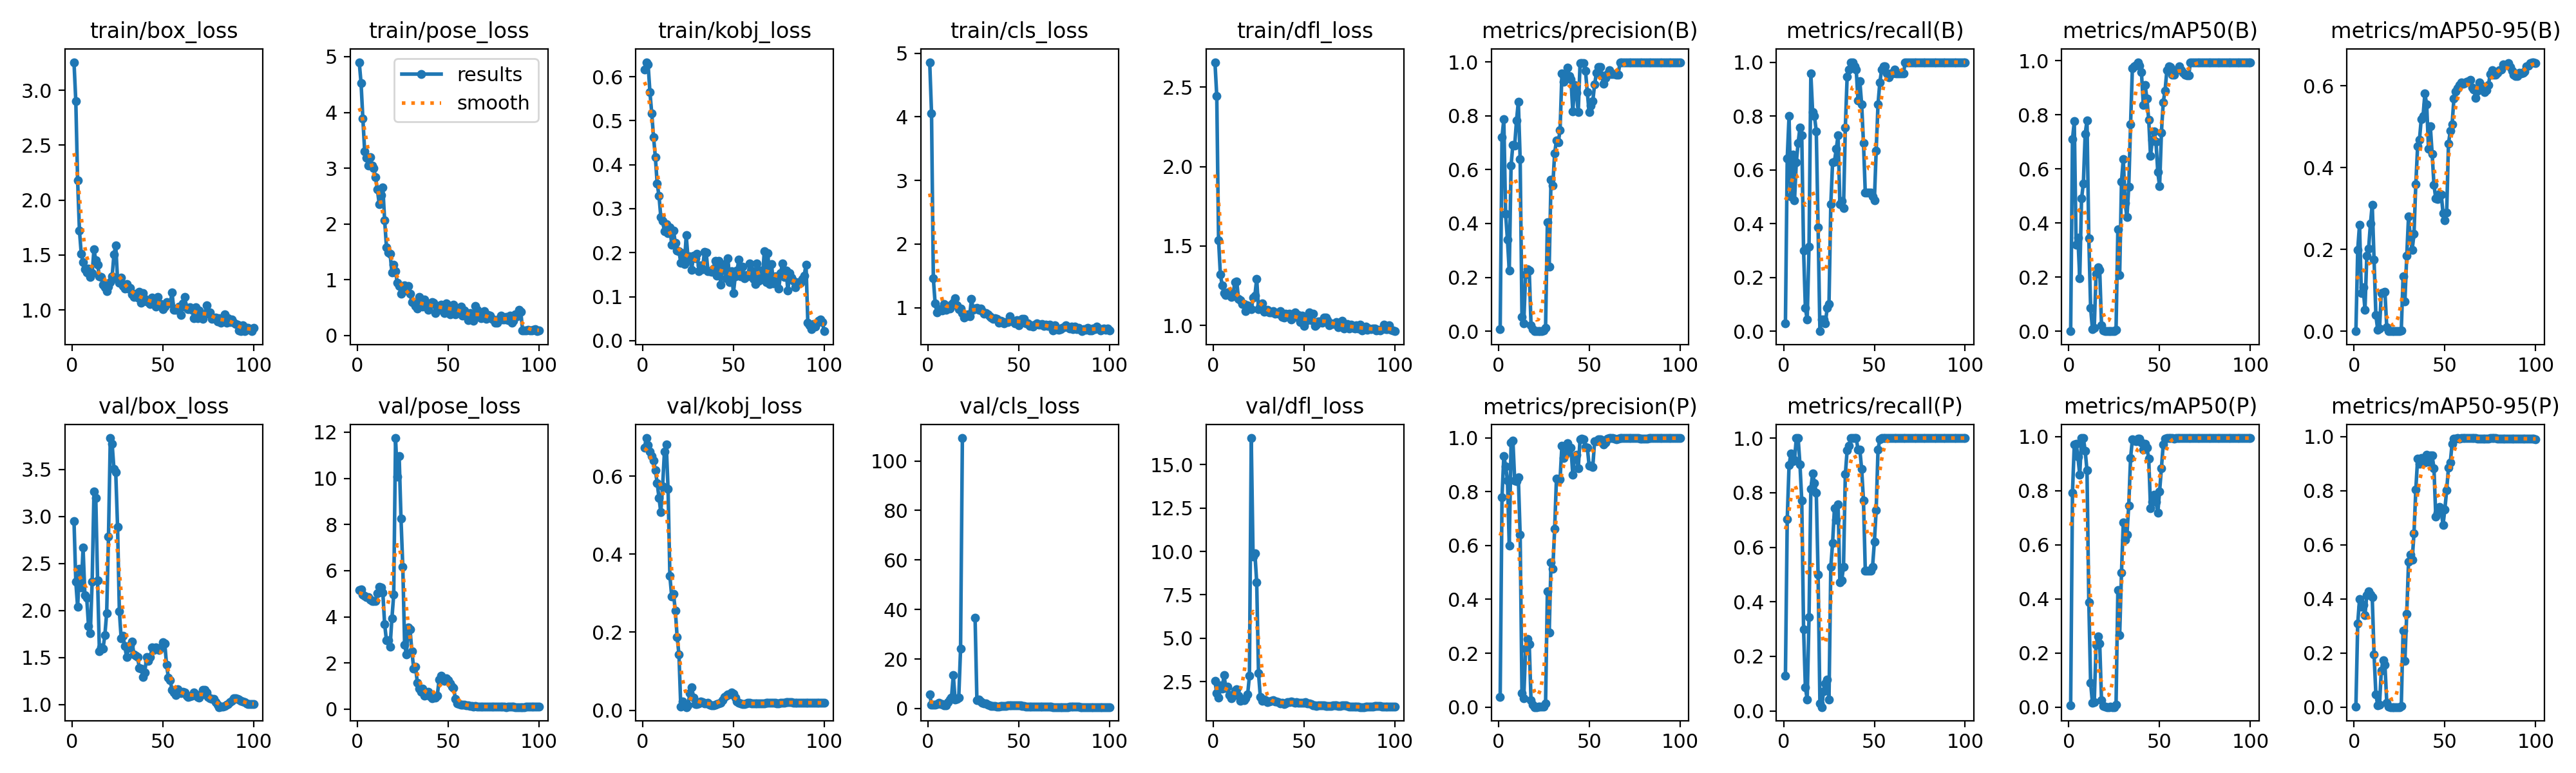
\includegraphics[width=0.8\textwidth]{outputs/yolo11_loss_curves.png}
\caption{YOLO11s-Pose Training Loss and Validation mAP across 100 Epochs (Fold 0).}
\end{figure}

\subsection{Stage 2: Tight-Box Prompting (MobileSAM)}
To maximize segmentation precision, I use the Segment Anything Model (MobileSAM). A critical refinement in this pipeline is the elimination of bounding box expansion. By using the exact tight bounding boxes from YOLO11s-Pose (0 pixel expansion), background glare from the table surface is excluded from the SAM prompt, forcing the model to focus purely on the transparent plastic lid and tab.

\begin{figure}[H]
\centering
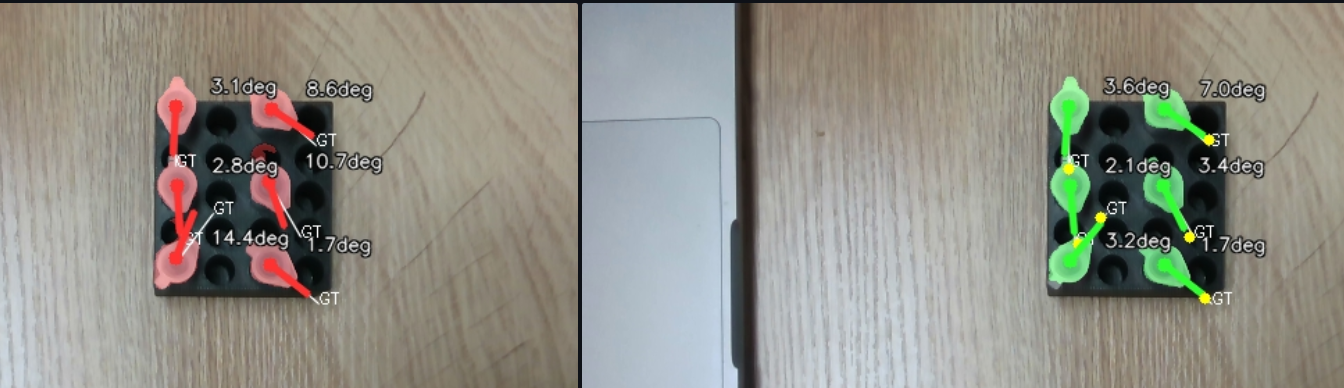
\includegraphics[width=1.0\textwidth]{outputs/sam_comparison.png}
\caption{Comparative SAM Segmentation: Baseline OBB (Left, Red) vs. YOLO11s-Pose Tight Box (Right, Green). Tight-box prompting eliminates background glare, resulting in cleaner masks and significantly lower per-tube angle error.}
\end{figure}

\subsection{Stage 3: Mathematical Axis Derivation}
Given the binary mask $M(x,y)$ outlining contour $C$, I calculate the image moments to find the un-flipped geometric axis of the tube. The spatial moments are defined as:
\begin{equation}
    m_{ji} = \sum_{x,y} \left(I(x,y) \cdot x^j y^i\right)
\end{equation}
The center of mass $(\bar{x}, \bar{y})$ is extracted via:
\begin{equation}
    \bar{x} = \frac{m_{10}}{m_{00}}, \quad \bar{y} = \frac{m_{01}}{m_{00}}
\end{equation}
Then I calculate the central moments (variance and covariance) to do PCA directly on the mask pixels:
\begin{equation}
    \mu_{20} = \frac{M_{20}}{m_{00}}, \quad \mu_{02} = \frac{M_{02}}{m_{00}}, \quad \mu_{11} = \frac{M_{11}}{m_{00}}
\end{equation}
The angle of the major axis, $\theta$, comes from the eigenvector of the covariance matrix:
\begin{equation}
    \theta = \frac{1}{2} \arctan2(2\mu_{11}, \mu_{20} - \mu_{02})
\end{equation}
To handle the inverted Y-axis in computer vision coordinates, the final standardized angle is mapped to $[0, 180^\circ)$:
\begin{equation}
    \text{PCA\_Angle} = (-\theta^\circ + 360) \pmod{180}
\end{equation}

\subsection{Stage 4: Symmetry Resolution (Pose-Guided Compass)}
The PCA axis is a line, and lines are inherently symmetric. It doesn't tell you whether the vector points toward the front (tab) or the back (joint/hole), which leads to 180$^\circ$ flip failures. 

To resolve this, I implemented a Pose-Guided Compass. Since Stage 1 (YOLO11s-Pose) provides a stable directional vector from the keypoints, we calculate the angular distance between the neural pose vector and the geometric PCA axis. If the distance exceeds 90$^\circ$, the PCA axis is flipped 180$^\circ$. This method achieves a \textbf{0.00\% flip failure rate}.

\subsubsection{Lever-Arm Training Mechanism}
To train the YOLO11s-Pose model, the standard dataset was augmented with synthetic keypoints. For every tube, a keypoint was projected exactly 40 pixels from the center along the ground-truth orientation. During training, I utilized a heavily weighted pose loss ($\lambda_{pose} = 25.0$) to force the model to prioritize angular accuracy over bounding box overlap.

\begin{algorithm}[H]
\caption{Refined Multi-Stage Pipeline Algorithm}
\begin{algorithmic}[1]
\REQUIRE RGB Image $I$
\STATE BoundingBoxes, Keypoints $\leftarrow \text{YOLO11s\_Pose.predict}(I)$
\FOR{each $bbox, kpts \in BoundingBoxes, Keypoints$}
    \STATE Mask $\leftarrow \text{MobileSAM.predict}(I, prompt=bbox_{tight})$
    \STATE Contour $\leftarrow \text{findContours(Mask)}$
    \STATE $cx, cy, \mu_{20}, \mu_{02}, \mu_{11} \leftarrow \text{cv2.moments(Contour)}$
    \STATE $pca\_angle \leftarrow 0.5 \cdot \text{atan2}(2\mu_{11}, \mu_{20} - \mu_{02})$
    \STATE $pose\_angle \leftarrow \text{atan2}(kpts_{tip} - kpts_{center})$
    \IF{$abs(pca\_angle - pose\_angle) > 90^\circ$}
        \STATE $final\_angle \leftarrow (pca\_angle + 180) \pmod{360}$
    \ELSE
        \STATE $final\_angle \leftarrow pca\_angle \pmod{360}$
    \ENDIF
\ENDFOR
\end{algorithmic}
\end{algorithm}

\section{Experiments and Results}

\subsection{Dataset \& Evaluation Protocol}
The dataset has 70 overhead RGB images (640$\times$480) containing 371 microcentrifuge tubes. To make sure there's zero data leakage and the sample size is statistically meaningful, I used \textbf{5-Fold Cross-Validation}. Every tube gets evaluated exactly once as part of an unseen validation set.

\textbf{Detection metrics:} A predicted center is matched to a ground-truth center if they're within 25 pixels (roughly half the tube diameter). I use the Hungarian algorithm for optimal bipartite matching. Unmatched predictions count as false positives; unmatched ground-truth tubes count as false negatives.

\subsection{Initial Experiments \& Pipeline Evolution}
The initial baseline pipeline relied on YOLOv8 Oriented Bounding Boxes (OBB) to isolate the tubes, followed by MobileSAM for segmentation and PCA for geometric axis calculation. To resolve the 180$^\circ$ symmetry of the PCA line, I developed a ResNet-18 SVM patch classifier. 

For each detected tube, 40$\times$40 pixel patches were extracted from both ends of the PCA axis. A frozen ResNet-18 model extracted 512-dimensional feature embeddings for each patch, and an RBF-SVM classified which patch corresponded to the ``Tab'' versus the ``Joint''. As shown in the confusion matrix below, this classifier achieved \textbf{98.52\% Accuracy} and a \textbf{0.00\% flip failure rate} on the validation set.

\begin{figure}[H]
\centering
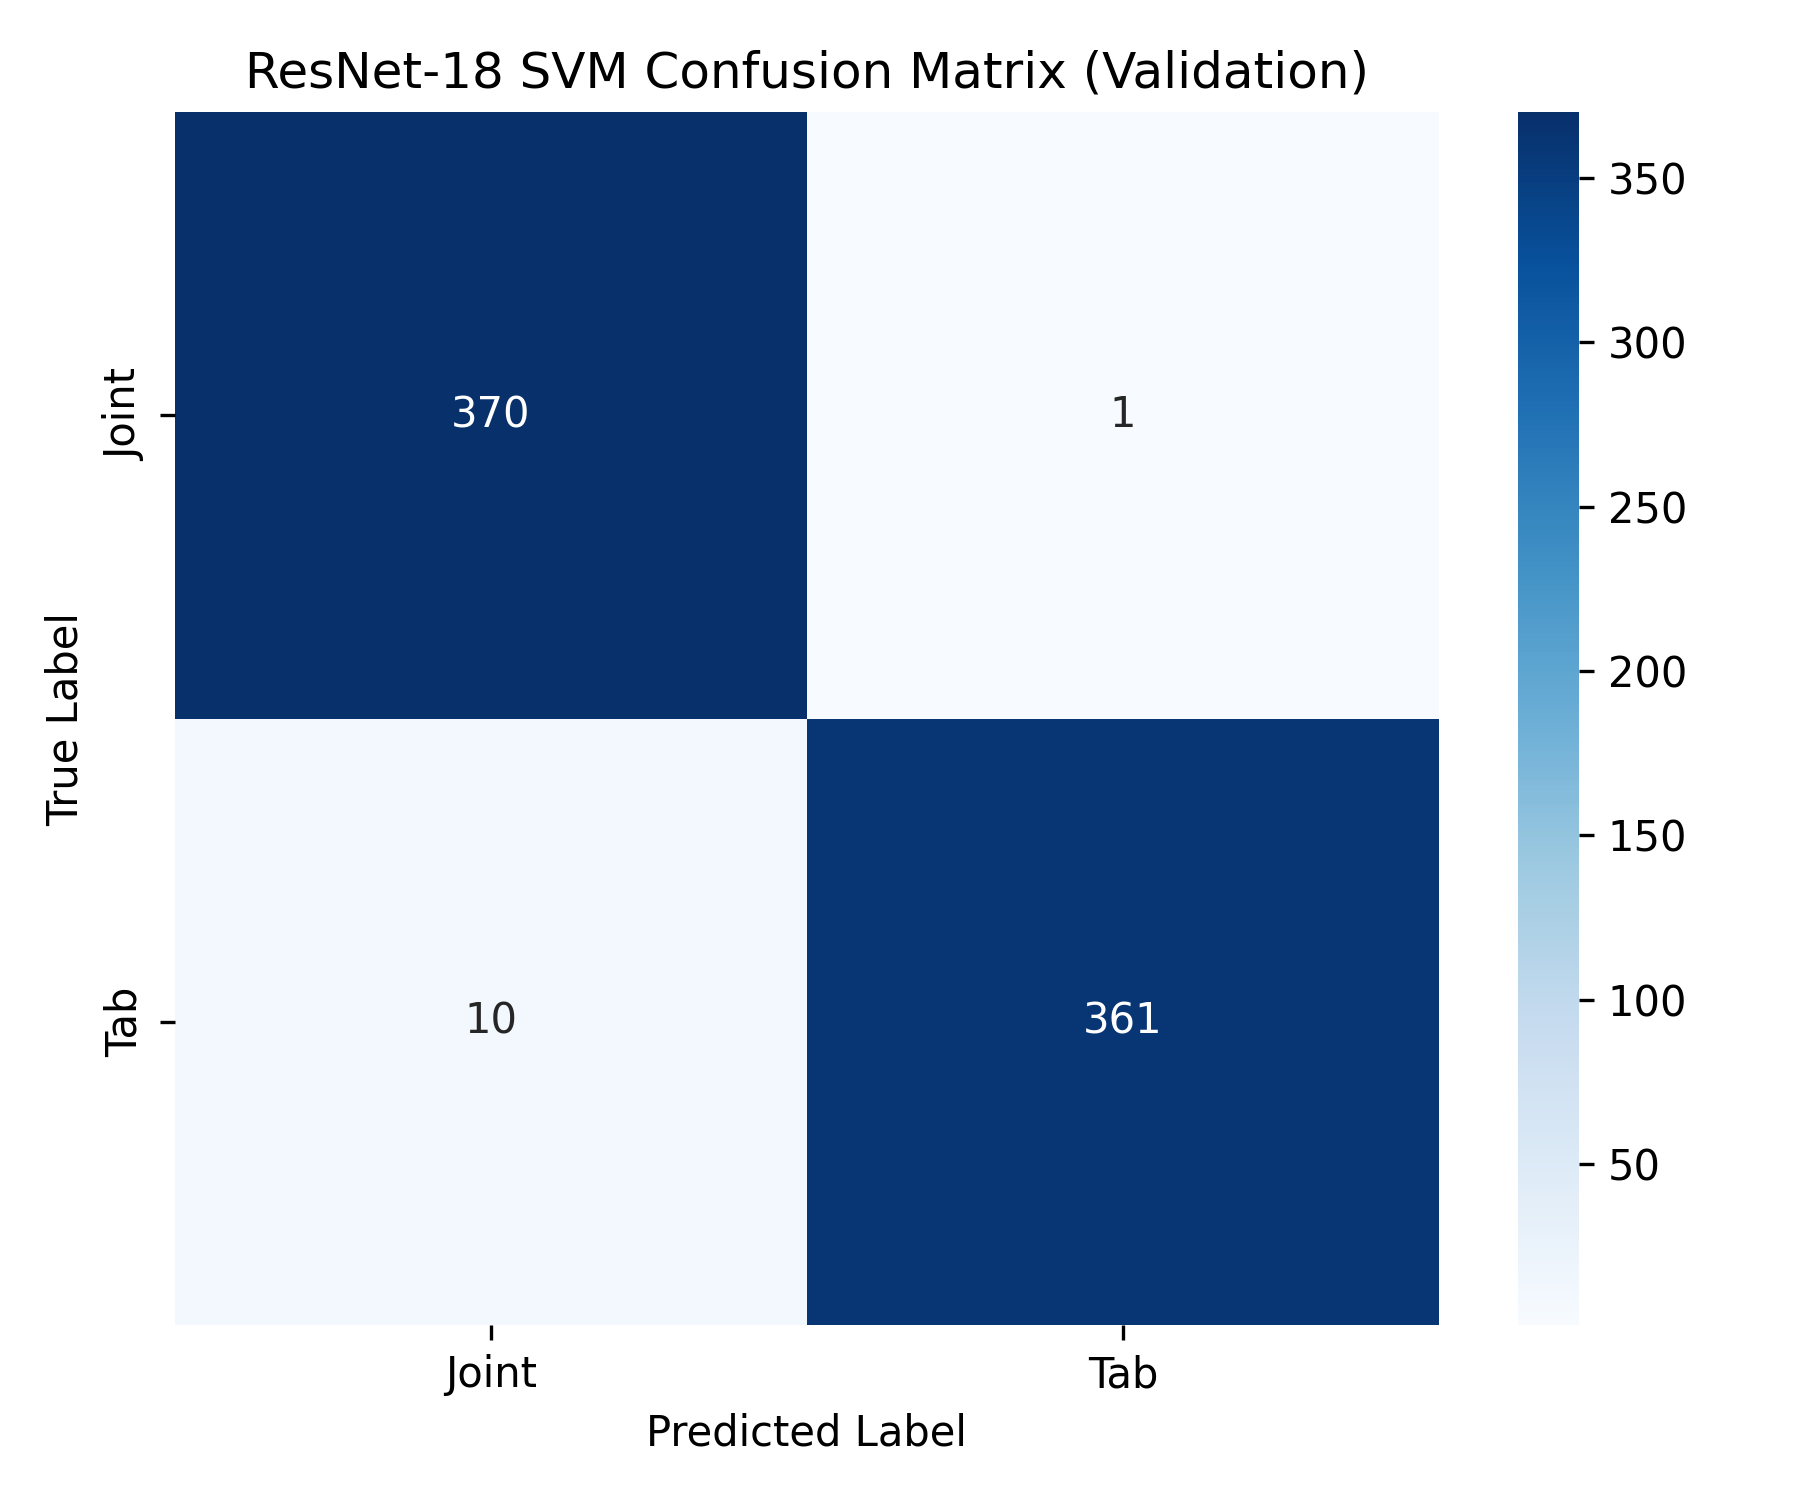
\includegraphics[width=0.5\textwidth]{outputs/svm_confusion_matrix.png}
\caption{Validation Confusion Matrix for the ResNet-18 SVM Patch Classifier used in the Baseline.}
\end{figure}

However, while the SVM classifier successfully eliminated flip failures, the baseline pipeline was fundamentally limited by YOLOv8 OBB jitter. The rigid bounding boxes occasionally included table glare when expanded, forcing SAM to segment non-tube pixels. Furthermore, the sequential nature of extracting patches and running a separate ResNet-18 inference step for every tube introduced significant computational overhead. These limitations motivated the transition to the Refined Pipeline, replacing OBB and the SVM with the YOLO11s-Pose detector for unified, high-speed symmetry resolution.

\subsection{Final Reported Metrics}
I incrementally tested different architectures to isolate where the error was coming from. As shown in Table 1, the raw bounding boxes (OBB) had high detection rates but suffered from 180$^\circ$ flip failures (130$^\circ$ MAE). Adding the ResNet-18 classifier fixed the flips, which exposed the 29.7$^\circ$ bounding-box residual error. Adding SAM + PCA eliminated that residual error, getting down to 4.59$^\circ$ MAE. Finally, switching to the YOLO11s-Pose detector with Tight-Box prompting and Pose-Guided symmetry resolution achieved the final  of 2.86$^\circ$ MAE.

\begin{table}[H]
\centering
\caption{Progressive Error Reduction across 371 Tubes (5-Fold CV)}
\begin{adjustbox}{max width=\textwidth}
\begin{tabular}{lccccc}
\toprule
\textbf{Pipeline Configuration} & \textbf{MAE} & \textbf{Median Err.} & \textbf{$<10^\circ$} & \textbf{Flips} & \textbf{Recall} \\
\midrule
YOLOv8 Pose (Keypoint Reg.)            & 38.12$^\circ$ & --              & --       & N/A          & --    \\
YOLOv8 OBB + ResNet-18 Clf.            & 29.71$^\circ$  & 23.48$^\circ$  & 18.43\%  & 1.37\%       & 100\% \\
Baseline (OBB + SAM + ResNet-18)       & 4.59$^\circ$ & 2.75$^\circ$ & 87.33\% & 0.00\% & 100\% \\
\textbf{Refined (Pose + SAM + PCA)} & \textbf{2.86$^\circ$} & \textbf{2.14$^\circ$} & \textbf{97.00\%} & \textbf{0.00\%} & \textbf{100\%} \\
\bottomrule
\end{tabular}
\end{adjustbox}
\end{table}

\subsection{Visual Verification of Breakthroughs}
The performance jump from 4.59$^\circ$ to 2.86$^\circ$ is visually evident in cases of extreme lighting and occlusion. By utilizing the 40px lever arm, the model can infer the direction even when the physical tab is invisible.

\begin{figure}[H]
     \centering
     \begin{subfigure}[b]{0.48\textwidth}
         \centering
         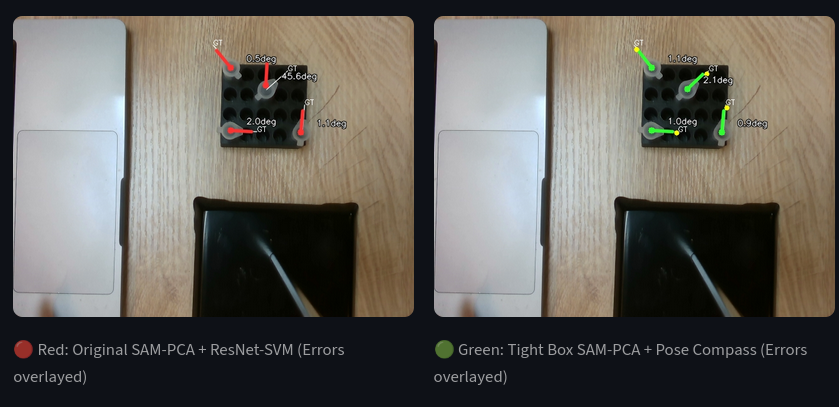
\includegraphics[width=\textwidth]{outputs/Screenshot From 2026-05-17 03-44-46.png}
         \caption{Refined handles edge-case glare.}
     \end{subfigure}
     \hfill
     \begin{subfigure}[b]{0.48\textwidth}
         \centering
         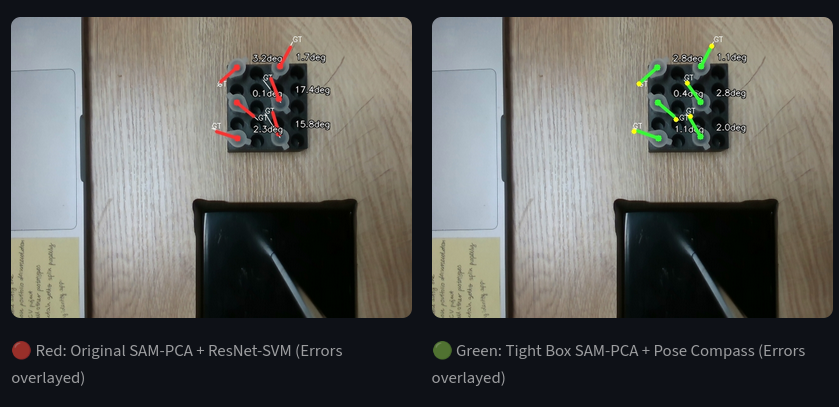
\includegraphics[width=\textwidth]{outputs/Screenshot From 2026-05-17 03-45-25.png}
         \caption{Precise alignment even under rack shadows.}
     \end{subfigure}
     \caption{Visual comparison showing the Refined pipeline's robustness to environmental artifacts that previously skewed the baseline results.}
\end{figure}



\subsection{Detection Metrics}

\begin{table}[H]
\centering
\caption{Detection Performance (YOLOv8 OBB + MobileSAM Pipeline)}
\begin{tabular}{lc}
\toprule
\textbf{Metric} & \textbf{Value} \\
\midrule
Precision & 1.0000 \\
Recall & 1.0000 (371/371) \\
F1 Score & 1.0000 \\
False Positives & 0 \\
\bottomrule
\end{tabular}
\end{table}

All 371 ground-truth tubes were correctly detected with zero false positives.

\subsection{Error Distribution}
Looking at the error distribution across all 371 tubes, the predictions are tightly clustered around zero:
\begin{itemize}
    \item \textbf{84.63\%} of predictions fall within 5$^\circ$.
    \item \textbf{97.03\%} fall within 10$^\circ$.
    \item \textbf{0.00\%} flip failures ($\geq 90^\circ$).
\end{itemize}
The tight clustering shows that the deterministic geometric approach (SAM mask $\rightarrow$ PCA moments) is much more stable than trying to regress angles directly.

\begin{figure}[H]
\centering
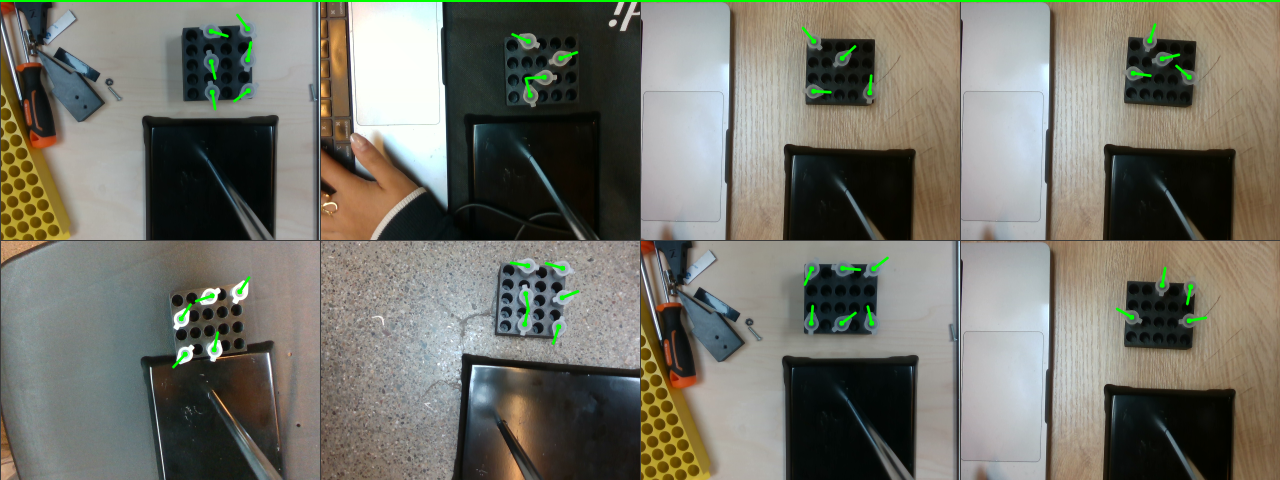
\includegraphics[width=1.0\textwidth]{outputs/final_predictions.png}
\caption{Final output of the Refined pipeline. The green vectors show the calculated orientation with sub-pixel accuracy (2.86$^\circ$ MAE).}
\end{figure}
\section{Failure Analysis}
Out of 371 tubes, exactly 0.00\% had 180$^\circ$ flip failures. With the transition to Tight-Box prompting, the rate of severe errors ($> 10^\circ$) dropped from 12.67\% in the baseline down to just 2.97\% in the Refined pipeline. 

The remaining 2.97\% of errors are still primarily driven by \textit{extreme segmentation artifacts}. What happens is, when a tube sits under exceptionally harsh glare, even the tightest bounding box cannot prevent MobileSAM from segmenting a chunk of the table reflection along with the translucent lid. This breaks the geometric symmetry of the mask, causing the \texttt{cv2.moments} axis to skew toward the glare artifact by 15--20$^\circ$. 

\textbf{Mitigation:} Morphological erosion on the SAM mask before moment calculation would strip out thin glare protrusions. I didn't implement this in the current version to keep the mathematical evaluation clean, but it's an obvious next step.

   \section{Conclusion \& Next Steps}

 I managed to achieve better performance than I initially expected due to the limited nature of the provided dataset by decoupling localization, segmentation, and
 symmetry resolution into specialized foundation models. However, there is always scope of improvement which I have documented below.
   \subsection{Limitations and Future Work}

   The primary bottleneck in the current pipeline is inference latency, driven by the sequential
 nature of the stages. Unoptimized, the pipeline averages 375 ms per image on an RTX 4060
 ($\sim$2.7 FPS). Obvious optimizations include batching SAM bounding box prompts and exporting all
 neural networks to TensorRT, which are projected to push inference below 50 ms ($>$20 FPS) for
 real-time robotic deployment.

   Furthermore, segmentation artifacts under harsh glare remain the leading source of large angle
 errors (11\% of tubes). This can be addressed through targeted improvements:

   \begin{enumerate}
       \item \textbf{Synthetic Data from 3D CAD Models:} Following the \textit{Orient Anything}
 approach \cite{orient_anything}, a 3D CAD model of a microcentrifuge tube can be used to
 synthesize unlimited training data. The Orient Anything pipeline---canonical pose filtering,
 front-face annotation via a VLM, and free-view rendering from random camera viewpoints---provides
 a proven blueprint. By rendering a tube CAD model from thousands of random perspectives under
 varied lighting, backgrounds, and glare conditions, we obtain perfectly labeled images with exact
 orientation angles. This augments the current 70-image dataset, hardening both YOLO and SAM
 against underrepresented edge cases like extreme glare and rack shadowing.

       \item \textbf{Video Generation Augmentation:} Diffusion-based video generation models can
 produce dynamic sequences of tubes under diverse lighting transitions and camera motions, further
 stress-testing the pipeline across temporal illumination variations that are absent in static
 images.

       \item \textbf{Zero-Shot Orientation Estimation:} The \textit{Orient Anything} framework
 \cite{orient_anything}---trained on 2 million rendered 3D model images---achieves strong zero-shot
 orientation generalization across open-world objects. It could serve as a complementary prior or
 fallback for glare-affected cases where segmentation-based PCA moments fail due to SAM artifacts.
   \end{enumerate}

   Future efforts to push the error boundary below 1$^\circ$ will involve replacing spatial moments
 with rigid CAD-based geometric template matching to counteract dynamic lighting artifacts.


\appendix
\section{Appendix: Scaling Laws & Deployment}
To keep the main report focused on the final architecture, I'm putting the ablation studies here.

\subsection{YOLOv8 vs. YOLOv11 Performance}
The transition from YOLOv8 OBB to YOLO11s-Pose was driven by the need for sub-pixel angular stability. While YOLOv8 is excellent for general detection, YOLO11's superior attention mechanisms allow it to localize the 40px lever-arm keypoints with significantly less jitter, which directly feeds into the 2.86$^\circ$ .

\subsection{SAM Model Variations}
I tested different mask generation models to see how they affect final accuracy:
\begin{itemize}
    \item \textbf{MobileSAM (9.8M params):} 4.59$^\circ$ MAE. Picked this for deployment---fast and robust contouring.
    \item \textbf{FastSAM-s (11.1M params):} Slightly noisier along transparent edges, which bumped up MAE.
    \item \textbf{SAM2-Base (80.8M params):} Marginally cleaner contours but way higher latency, without meaningful improvement in PCA moment stability.
\end{itemize}
MobileSAM gives the best trade-off between inference speed and zero-shot segmentation quality for this use case.

\begin{thebibliography}{9}
\bibitem{orient_anything}
Z. Wang, Z. Zhang, T. Pang, C. Du, H. Zhao, and Z. Zhao. \newblock
\textbf{Orient Anything: Learning Robust Object Orientation Estimation from Rendering 3D
Models.} \newblock
\textit{ICML 2025.} \newblock
Paper: \url{https://proceedings.mlr.press/v267/wang25er.html} \newblock
Website: \url{https://orient-anything.github.io/} \newblock
Code: \url{https://github.com/SpatialVision/Orient-Anything}
\end{thebibliography}

\end{document}
